\documentclass[12pt]{article}
\usepackage[utf8]{inputenc}
\usepackage{graphicx}
\usepackage{multicol}
\usepackage{listings}
\usepackage{amsmath}
\graphicspath{ {./images/} }
\usepackage{amssymb}
\usepackage[htt]{hyphenat}

\usepackage{hyperref}
\hypersetup{
    colorlinks=true,
    linkcolor=blue,
    filecolor=magenta,      
    urlcolor=cyan,
}

\usepackage{xcolor}

\definecolor{codegreen}{rgb}{0,0.6,0}
\definecolor{codegray}{rgb}{0.5,0.5,0.5}
\definecolor{codepurple}{rgb}{0.58,0,0.82}
\definecolor{backcolour}{rgb}{0.95,0.95,0.92}
\definecolor{codeorange}{rgb}{1,0.64,0}

\lstdefinestyle{mystyle}{
    backgroundcolor=\color{backcolour},   
    commentstyle=\color{codegreen},
    keywordstyle=\color{magenta},
    numberstyle=\tiny\color{codeorange},
    stringstyle=\color{codepurple},
    basicstyle=\ttfamily\footnotesize,
    breakatwhitespace=false,         
    breaklines=true,                 
    captionpos=b,                    
    keepspaces=true,                 
    numbers=left,                    
    numbersep=5pt,                  
    showspaces=false,                
    showstringspaces=false,
    showtabs=false,                  
    tabsize=2
}

\lstset{style=mystyle, breaklines=true, postbreak=\mbox{\textcolor{red}{$\hookrightarrow$}\space}}

\title{\vspace{-1cm}The Tubelight Simulation\\
\large Assignment 6\\
\large EE2703 - Applied Programming Lab}
\author{Abhigyan Chattopadhyay \\
EE19B146}
\date{30th March 2021}
\usepackage[margin=0.75in]{geometry}

\begin{document}
\maketitle
\tableofcontents
\pagebreak
\section{The Problem at Hand}
We will simulate a Tube light using a Monte-Carlo simulation technique, and obtain the distribution of electrons and the light intensity as a function of position. 

We will also tabulate the intensity of light emitted as a function of position.

\subsection{Explaining The Physics}
When a sufficiently energized electron strikes an atom, it causes the atom to ionize and gain some energy, which is then lost as a photon when the atom tries to regain its neutral state. This packet of light is emitted as soon as the electron hits the atom.

In a tube light, we have an electric field which accelerates electrons that are generated at the cathode, which gain energy as they pass through the tube, and once their velocity is above a certain threshold velocity, they are able to excite atoms and cause them to release photons.

The following equations of motion are followed by the electrons in the tube:

$$v_i = u_i + at$$
$$x_e = u_i t + \frac{1}{2} a t^2$$
$$u_i>u_0 \implies p\text{ probability of } h\nu \text{ emitted}$$
(Here $u_0$ is the threshold velocity for photon emission)

We will assume $a$ to be 1 in this simulation, and 1 unit of time to be the smallest possible discrete unit of time.

\subsection{What is a Monte-Carlo Simulation}

A Monte-Carlo simulation is one where repeated sampling is used to obtain numerical results.

Here, we will generate a random number of electrons, and choose some of them randomly to be able to release a photon upon collision, using random number generators in \texttt{numpy}.

We are using it here to easily enable us to simulate these electrons as they generate light in the tube. The idea is to get accurate results that can be generalized over a number of different types of tube lights.

\pagebreak
\section{Monte-Carlo Simulation}

\subsection{Parameters}
We have 6 main parameters here, namely:

\begin{itemize}
    \item $n$    (int)   = spatial grid size
    \item $M$    (int)   = number of electrons injected per turn
    \item $M_{sig}$ (int)   = standard deviation for electrons injected per turn
    \item $n_k$   (int)   = number of turns to simulate
    \item $u_0$   (float) = threshold velocity required to excite an atom
    \item $p$    (float) = probability that a collision results in an excited atom
\end{itemize}

We will use these to effectively accommodate different types and lengths of tubes ($n$), cathodes ($M$and $M_{sig}$), electric fields and different gases present in the tubes ($p$ and $u_0$).

$n_k$ is essentially the amount of time we want to simulate the tube light for. It is essentially $n_k$ times the shortest discrete unit of time in the simulation.

These parameters can be entered in the terminal as command line arguments, and if left empty, they default to:

\begin{itemize}
    \item $n = 100$
    \item $M = 5$
    \item $M_{sig} = 1$
    \item $n_k = 500$
    \item $u_0 = 5$
    \item $p = 0.25$
\end{itemize}

Help on adding command line arguments can be accessed by writing the name of the script followed by \texttt{help}:

\begin{center}
For eg: \texttt{python Assignment\_6.py help}
\end{center}
\pagebreak
\subsection{Setting up the Simulation Environment}
Now that we have our parameters handy, we can start setting up the environment.

The first thing to set up would be a few vectors to store the absolute position of the electrons in the tube, their velocities, and their displacements with respect to their last positions.

We do this as follows:
\begin{lstlisting}[language=Python]
import numpy as np
...
def montecarlo(n,M,Msig,nk,u0,p,accurateMode=False):
    xx = np.zeros((n*M),dtype=float)
    u  = xx.copy()
    dx = xx.copy()
\end{lstlisting}

We set them to have \texttt{n*M} elements, although that is too much, but it enables us to work easily.

We also need a set of lists to store the locations of the photons that get emitted, and the positions and velocities of the electrons at each stage, so that we can make a population plot and phase-space plot later.

\begin{lstlisting}[language=Python]
    I = []
    X = []
    V = []
\end{lstlisting}

\texttt{I} hold the position of the photon generation, \texttt{X} holds the positions of the electrons, and \texttt{V} holds their velocities.

\subsection{Iterating the Simulation}
The simulation is done in 3 main steps:

\begin{enumerate}
    \item Advancing the electrons from their current locations
    \item Handling collisions and photon generation
    \item Injecting new electrons
\end{enumerate}

This is done as follows:

\subsubsection{Advancing the Electrons}
First, we need to set up some rules with the arrays that we have made.
In the \texttt{xx} array, a position of 0 indicates that the electron is not present in the tube. A position of $[1,n-1]$ indicates that it is present in the tube.

Since we considered the acceleration to be 1 and are doing it for 1 time step at a time, we have:

$$dx = u\cdot1 + 0.5\cdot 1 \cdot 1^2$$
$$xx_{new} = xx_{prev} + dx$$
$$u_{new} = u_{prev} + 1\cdot 1$$

And as soon as it crosses $n-1$, we need to reset the electron's location and velocity back to 0 to indicate that it has left the tube.

With this in mind, we do the following:

\begin{lstlisting}[language=Python]
    for k in range(nk):
        # Step 1: Advancing the electrons
        # Step 1.1: Finding the locations of the active electrons
        ii = np.where(xx>0)
        # Step 1.2: Adding all the electron positions to the X and V vectors
        X.extend(xx[ii].tolist())
        V.extend( u[ii].tolist())
        # Step 1.3: Adjusting the displacement, position and velocity using the equations of motion
        dx[ii]  =  u[ii] + 0.5
        xx[ii] += dx[ii]
        u[ii]  += 1
        # Step 1.4: Setting the electrons that reached the anode to inactive
        u[np.where(xx>=n)] = 0
        xx[np.where(xx>=n)] = 0
\end{lstlisting}

\subsubsection{Handling collisions and photon generation}

Next, we handle all the possible collisions of energetic electrons with molecules of gas present in the tube.

An electron that has sufficient energy to collide may not always produce a photon, that is also generated via a random number generator, and must be less than the probability parameter, $p$.

Using this, we are able to find the location of photons being generated.

Here is the code used to achieve this:
\begin{lstlisting}[language=Python]
        #... continued from the for loop above
        # Step 2: Handling collisions and photon generation
        # Step 2.1: Select all electrons with velocity greater than threshold velocity
        kk = np.where(u>=u0)[0]
        # Step 2.2: Generate some electrons which excite the atoms
        ll = np.where(np.random.rand(len(kk))<=p)[0]
        kl = kk[ll]
        if accurateMode:
            # Step 2.3: Don't set the velocity of the electrons that collided to 0
            #u[kl] = 0
            # Step 2.4: Find the position of collision of these electrons
            dt = np.random.rand(len(kl))
            xx[kl]=xx[kl]-dx[kl]+((u[kl]-1)*dt+0.5*dt*dt)+0.5*(1-dt)**2 #accurate collision location
            u[kl]=1-dt #accurate velocity update
        else:
            # Step 2.3: Set the velocity of the electrons that collided to 0
            u[kl] = 0
            # Step 2.4: Find the position of collision of these electrons
            xx[kl]=xx[kl]-dx[kl]*np.random.rand(len(dx[kl]))
        
        # Step 2.5: Add all the excited atom locations to the list of photon positions
        I.extend(xx[kl].tolist())

\end{lstlisting}
\pagebreak
\subsubsection{Injecting new electrons}

This step involves using a random number generator, multiplying it with the standard deviation and adding it with the mean number of electrons generated per step, and then using this number to add a few new electrons at the cathode.

This is done by merely setting their positions to 1. The tricky part is putting the electrons into slots that aren't already occupied by active electrons.

\begin{lstlisting}[language=Python]
        #... continued from the for loop above
        # Step 3: Injecting new electrons
        # Step 3.1: Calculate number of electrons based on random number generator
        m = (np.random.randn())*Msig+M
        # Step 3.2: Choose min of free slots available and number of electrons from above
        freeslots = np.where(xx==0)[0]
        m = int(min(m,len(freeslots)))
        # Step 3.3: Set first m freeslot locations to 1
        xx[freeslots[:m]] = 1
\end{lstlisting}

And thus, we have our algorithm to iterate over the entire space of the tube light and make use of a large number of electron slots if needed.
\pagebreak
\subsection{Plotting the Outputs}
This section is fairly simple.

We first plot a histogram of the electron positions that we have stored over the various iterations, and the code and plot generated are below:

\begin{lstlisting}[language=Python]
import matplotlib.pyplot as plt
...
# Plotting the graphs
plt.figure(0)
plt.hist(X,n,edgecolor='black',linewidth=0.5)
plt.title("Population Plot of Electron Position")
plt.xlabel(r"$x\rightarrow$")
plt.ylabel(r"Number of Electrons$\rightarrow$")
plt.savefig("images/fig0.png",dpi=1000)
plt.show()
\end{lstlisting}

\begin{center}
    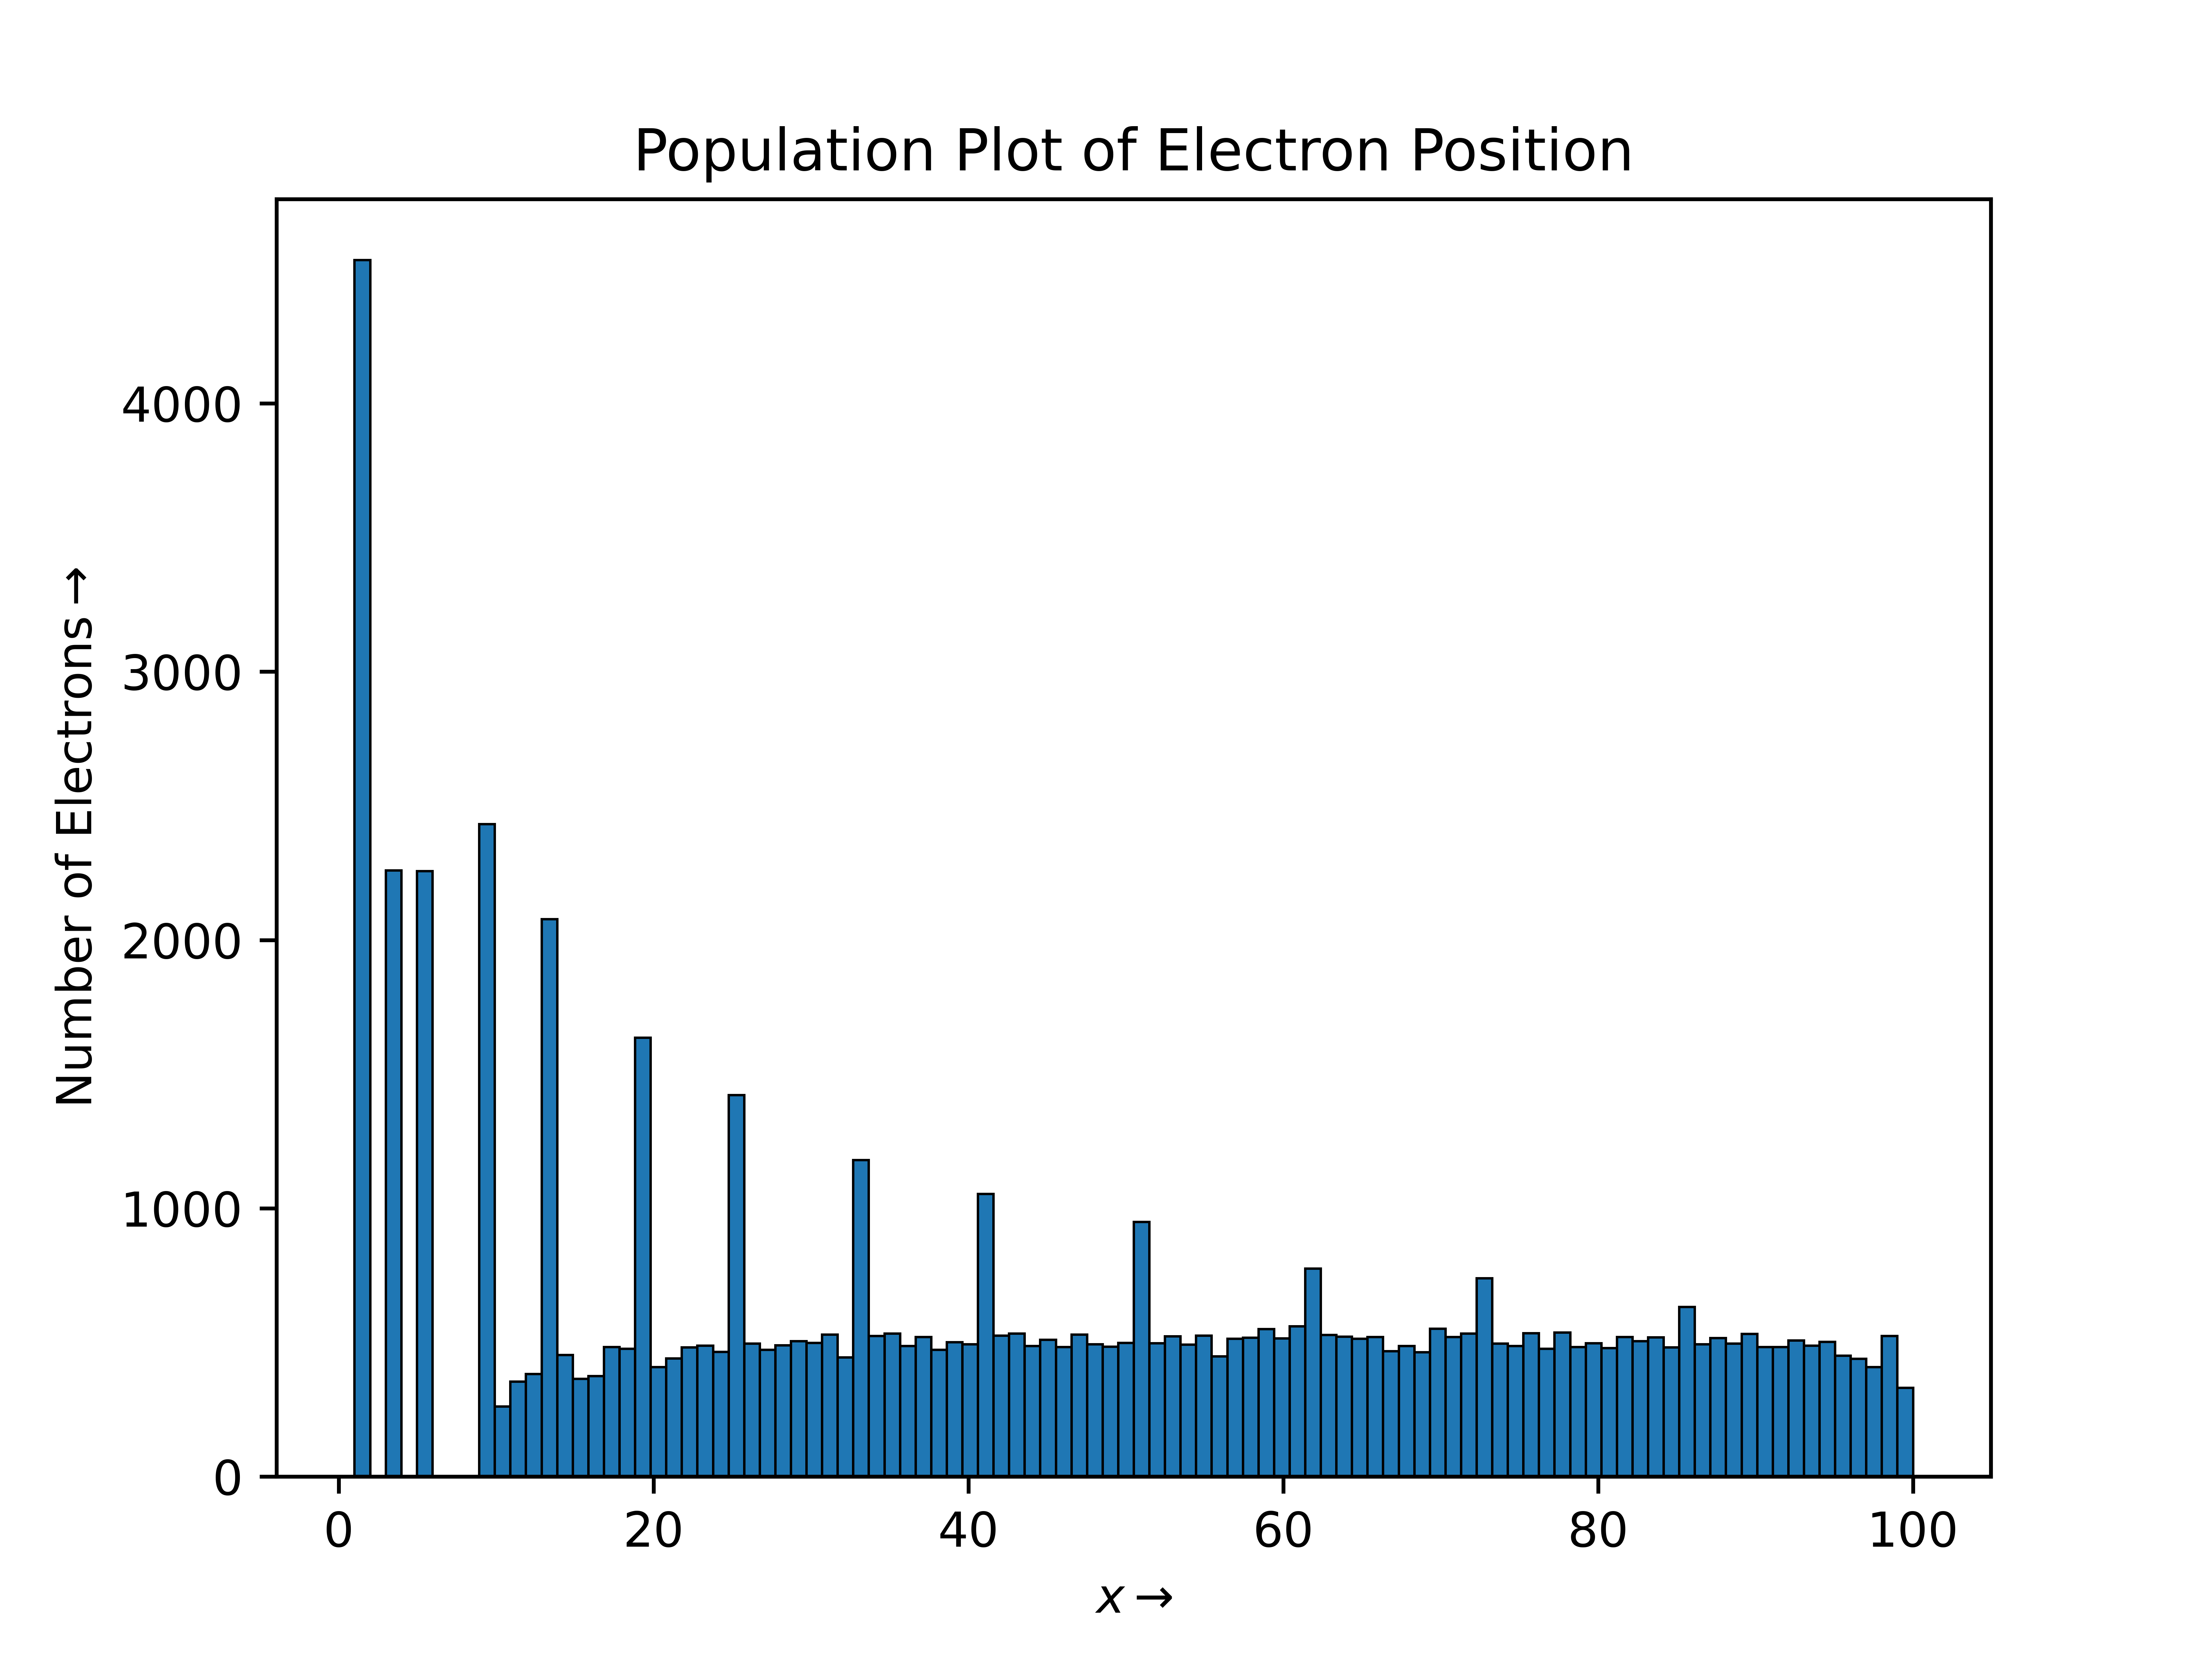
\includegraphics{images/fig0.png}
\end{center}

\pagebreak
\begin{lstlisting}[language=Python]
plt.figure(1)
counts,bins,_ = plt.hist(I,n,[0,n],edgecolor='black',linewidth=0.5)
plt.title("Population Plot of Intensity")
plt.xlabel(r"$x\rightarrow$")
plt.ylabel(r"Number of Photons Emitted ($\propto$ Intensity)$\rightarrow$")
plt.savefig("images/fig1.png",dpi=1000)
plt.show()
\end{lstlisting}

\begin{center}
    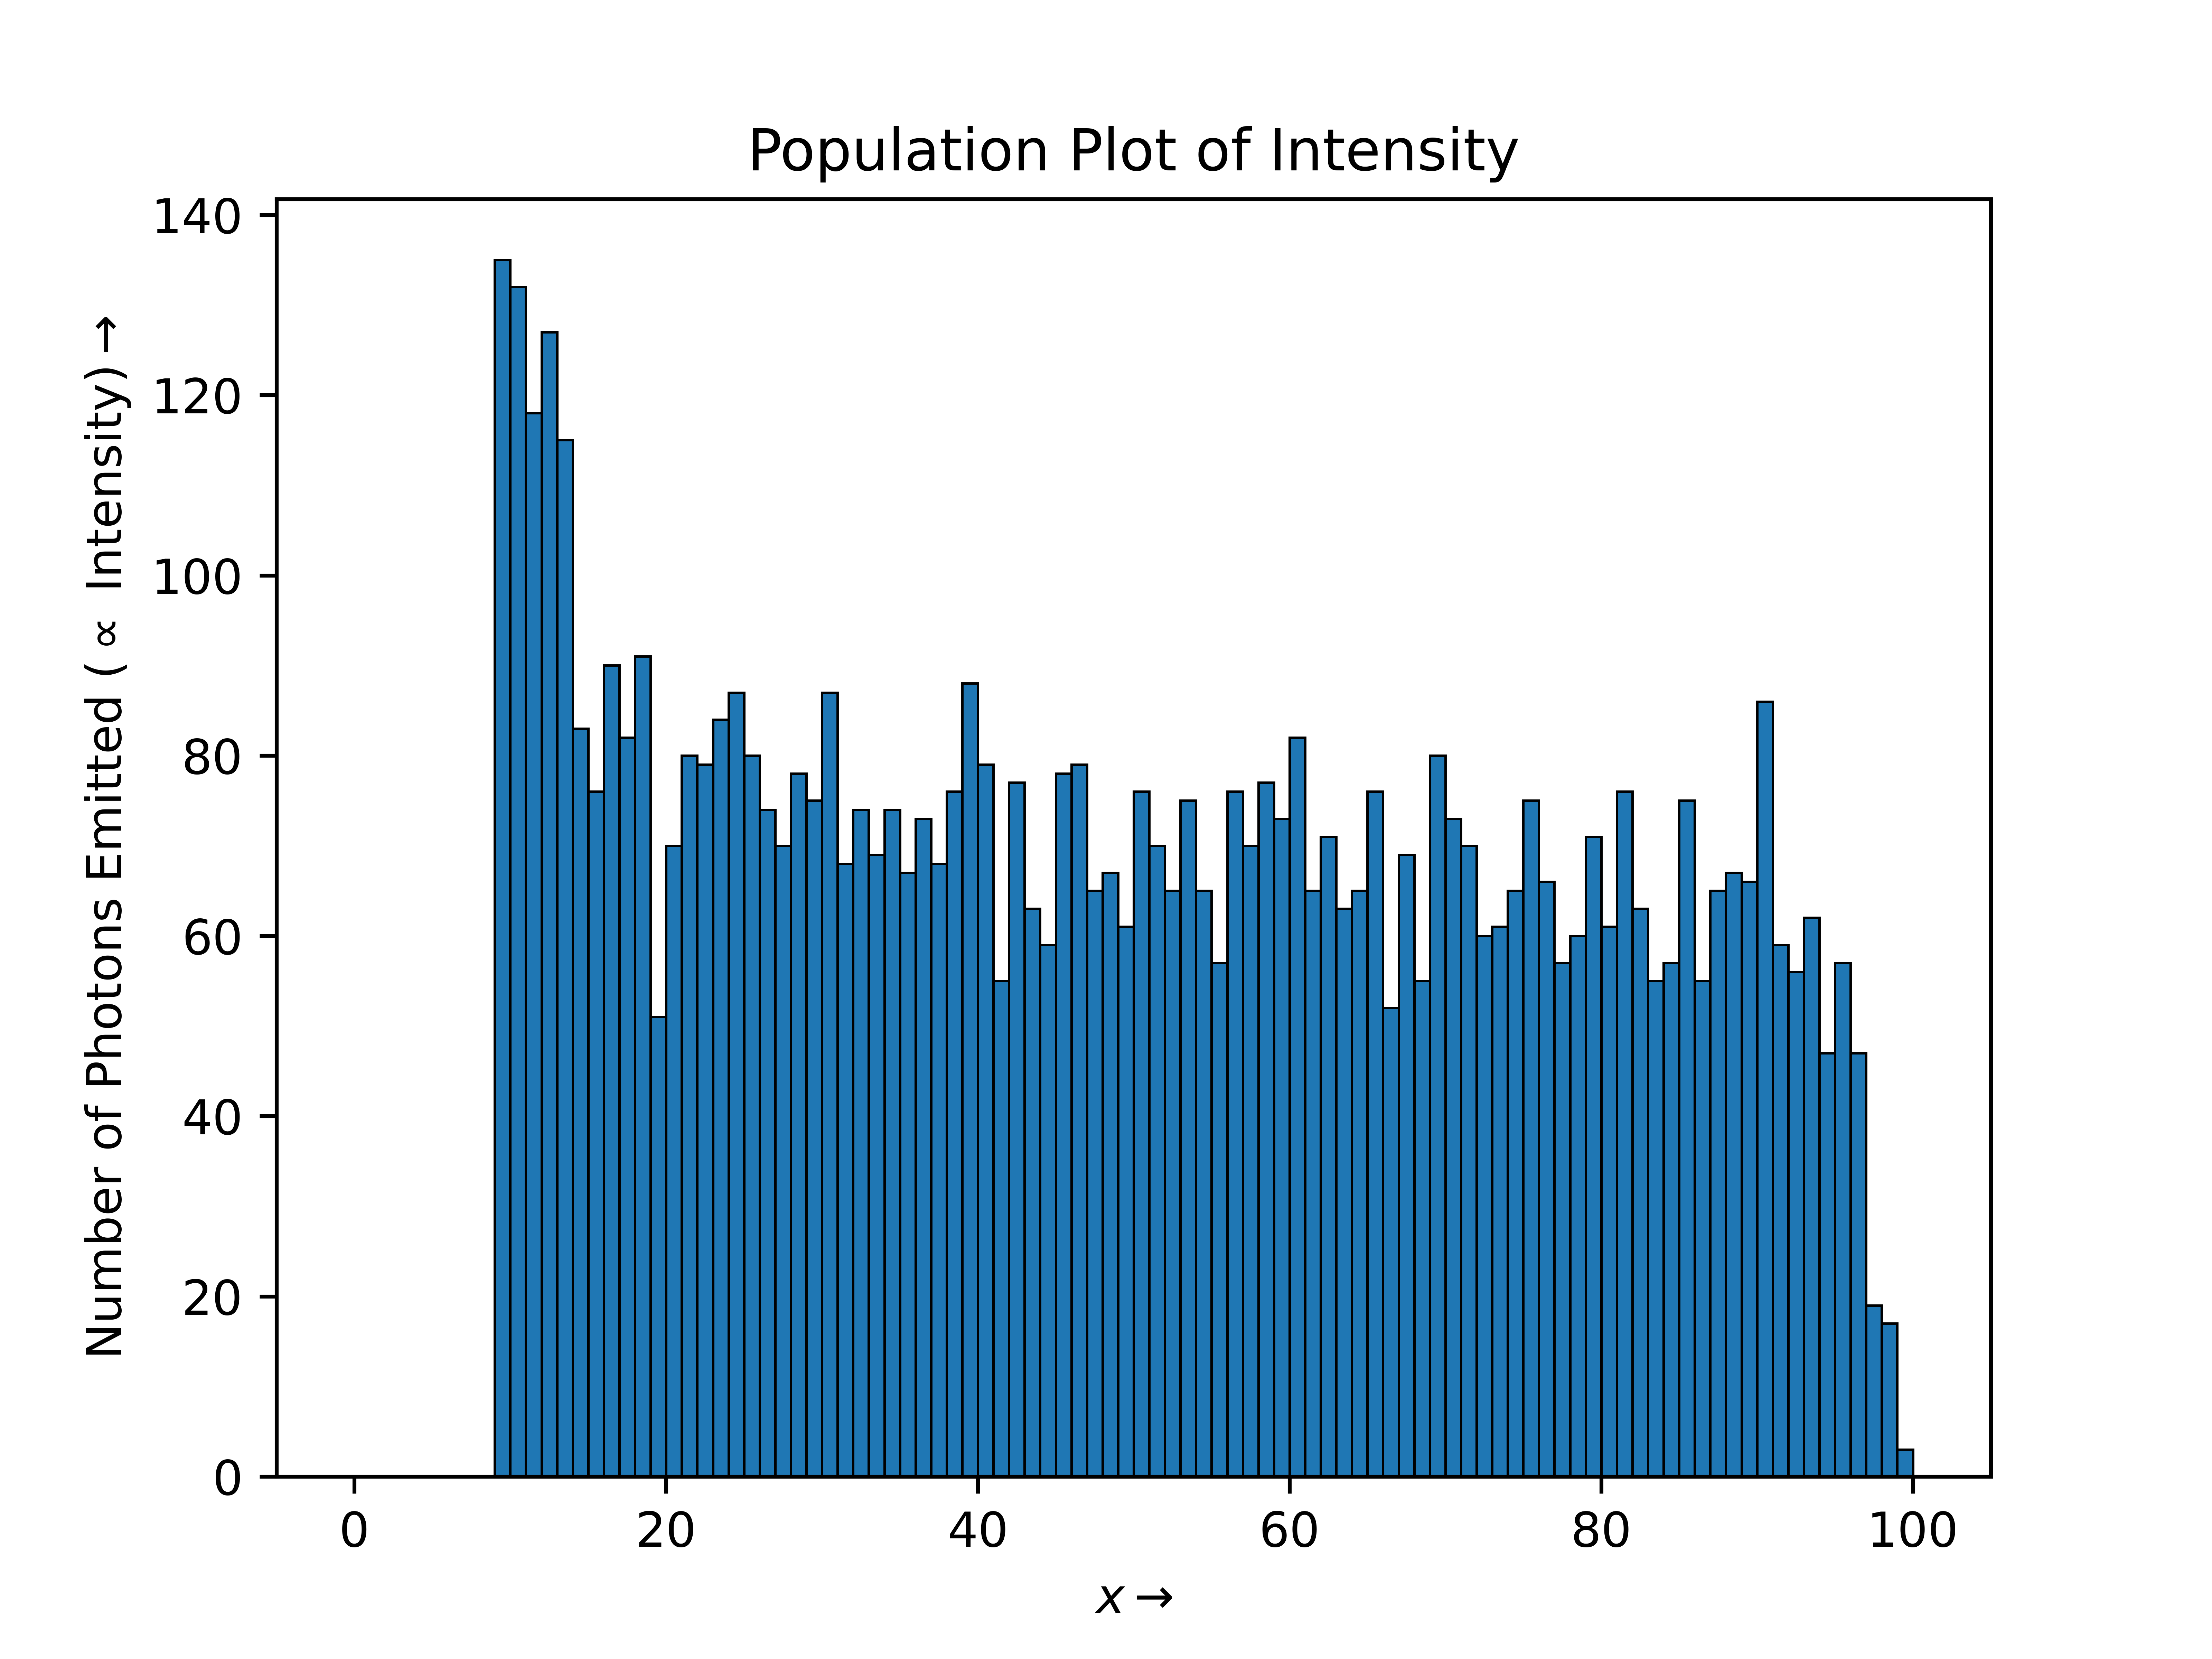
\includegraphics{images/fig1.png}
\end{center}

\pagebreak
\begin{lstlisting}[language=Python]
plt.figure(2)
plt.scatter(X,V,marker='^')
plt.title("Electron Phase Space")
plt.xlabel("$x$")
plt.ylabel("$v$")
plt.savefig("images/fig2.png",dpi=1000)
plt.show()
\end{lstlisting}

\begin{center}
    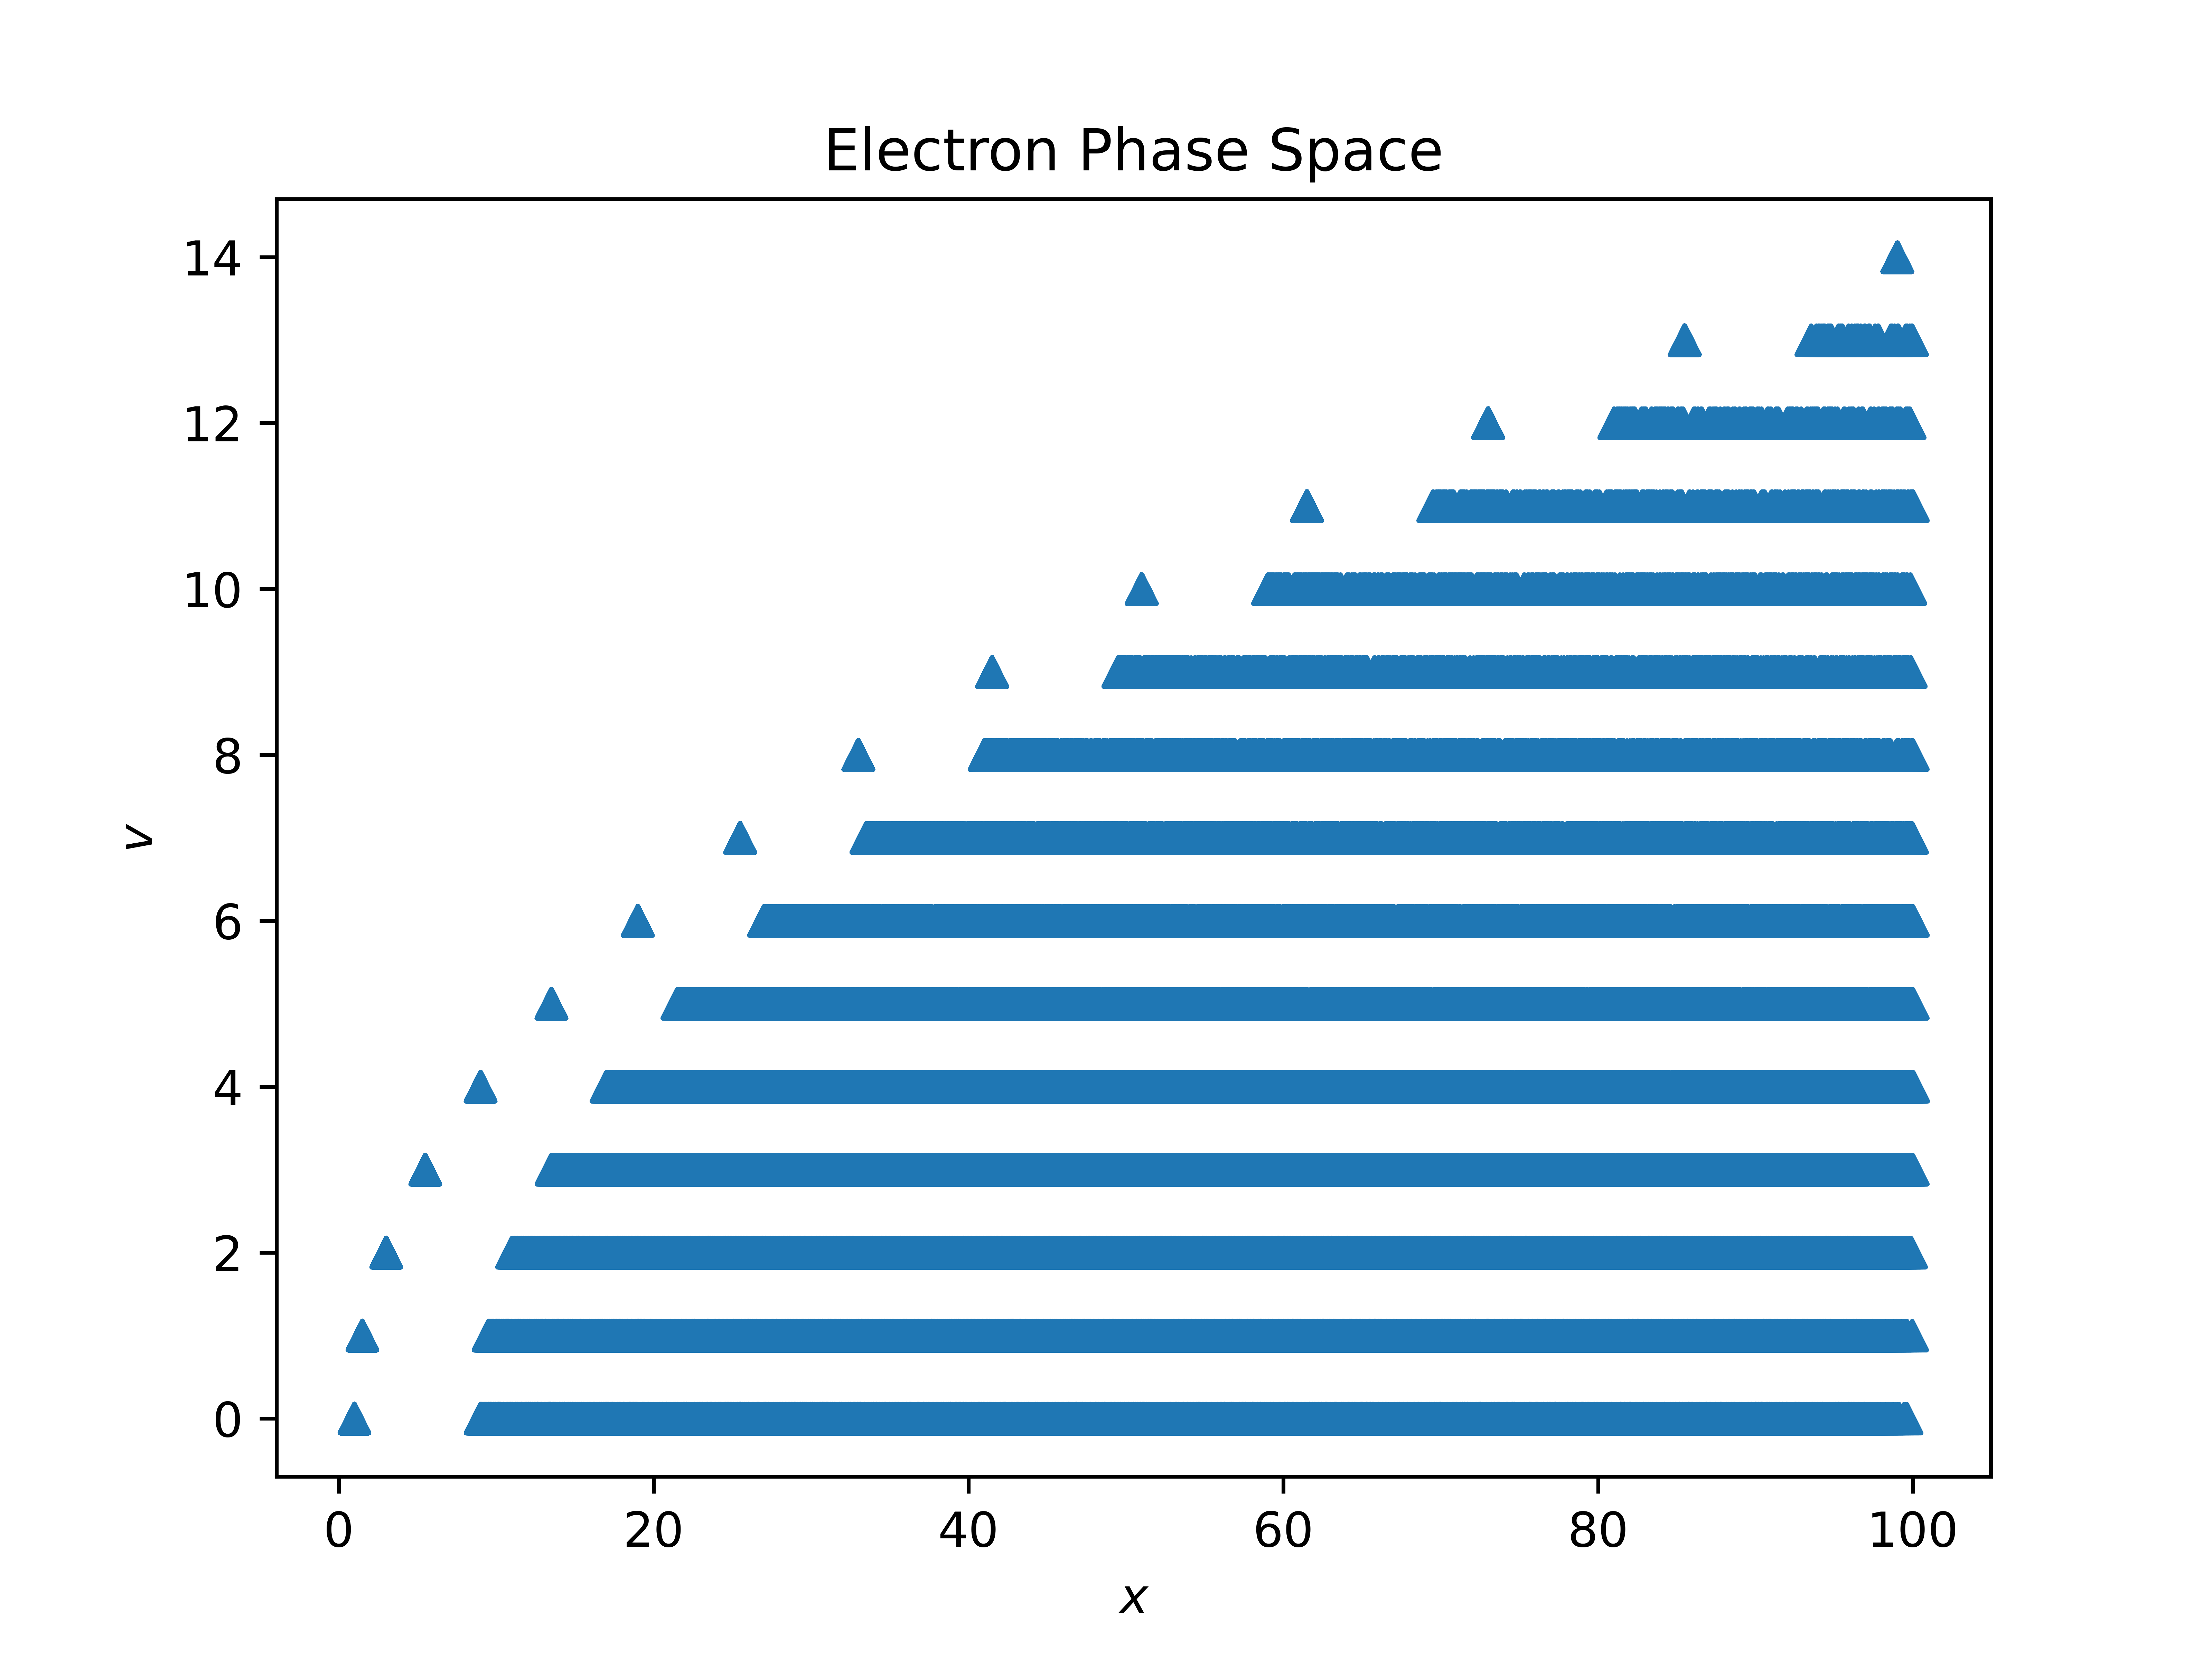
\includegraphics{images/fig2.png}
\end{center}

\subsection{Tabulating the intensity of light as a function of position}

For this section, we make use of the Python library: \texttt{tabulate}. It makes it a lot easy to print a tabular data.

We will use the bins and the counts that were generated in the previous diagram to make the tabulation easier.

\begin{lstlisting}[language=Python]
from tabulate import tabulate as tb
...
# Tabulating the data
xpos = 0.5*(bins[0:-1]+bins[1:])
print("Intensity data:")
print(tb(np.c_[xpos,counts],headers=['xpos','count']))
\end{lstlisting}
\pagebreak
This results in the following table:
\begin{multicols}{3}
\begin{verbatim}
Intensity data:
  xpos    count
------  -------
   0.5        0
   1.5        0
   2.5        0
   3.5        0
   4.5        0
   5.5        0
   6.5        0
   7.5        0
   8.5        0
   9.5      135
  10.5      132
  11.5      118
  12.5      127
  13.5      115
  14.5       83
  15.5       76
  16.5       90
  17.5       82
  18.5       91
  19.5       51
  20.5       70
  21.5       80
  22.5       79
  23.5       84
  24.5       87
  25.5       80
  26.5       74
  27.5       70
  28.5       78
  29.5       75
  30.5       87
  31.5       68
  32.5       74
  33.5       69
  34.5       74
  35.5       67
  36.5       73
  37.5       68
  38.5       76
  39.5       88
  40.5       79
  41.5       55
  42.5       77
  43.5       63
  44.5       59
  45.5       78
  46.5       79
  47.5       65
  48.5       67
  49.5       61
  50.5       76
  51.5       70
  52.5       65
  53.5       75
  54.5       65
  55.5       57
  56.5       76
  57.5       70
  58.5       77
  59.5       73
  60.5       82
  61.5       65
  62.5       71
  63.5       63
  64.5       65
  65.5       76
  66.5       52
  67.5       69
  68.5       55
  69.5       80
  70.5       73
  71.5       70
  72.5       60
  73.5       61
  74.5       65
  75.5       75
  76.5       66
  77.5       57
  78.5       60
  79.5       71
  80.5       61
  81.5       76
  82.5       63
  83.5       55
  84.5       57
  85.5       75
  86.5       55
  87.5       65
  88.5       67
  89.5       66
  90.5       86
  91.5       59
  92.5       56
  93.5       62
  94.5       47
  95.5       57
  96.5       47
  97.5       19
  98.5       17
  99.5        3
\end{verbatim}
\end{multicols}
\pagebreak
\section{Conclusions from first set}
We see that the tube light has a dark spot before $x=\frac{u_0^2}{2}$, which is consistent with the physics explanation that $v = \sqrt{2\cdot1\cdot x}$ and that $v>u_0$ for excitation.

From 0 to $\frac{u_0^2}{2}$, the electrons gain energy and then they collide after crossing the point with sufficient energy.

We also see that the phase plot is in the form of bands, but this is only because we have discretized the time and as a result every velocity is different from the other by only 1 unit.

We have not updated the velocity accurately after each collision, and hence this shape. There is a more accurate time and velocity update possible, which we will do next.

Also, it appears like it has a parabolic envelope, which is as expected, since $v^2 = 2x$. This envelope is of all the electrons that travelled straight from the cathode to anode without any collisions. The remaining collisions are evenly distributed below the envelope.

Finally, the electron population graph tells us that the electrons are in very large numbers near the cathode, and in the remaining space, they all are almost uniform, with a few peaks.

These peaks occur wherever the electrons have gained some energy but haven't yet crossed the threshold. These peaks are at the first few time steps that are experienced by these electrons. Most of the electrons reach the threshold velocity at approximately the same locations, and hence the peaks in the graph.

These peaks then smoothen out as we move towards the other end of the tube, as the number of electrons above the threshold increase.

\section{More accurate Velocity and Time Update}

The for loop remains almost the same with a few changes in step 2, which can be used by activating the \texttt{accurateMode} option of the \texttt{montecarlo} function.

This achieves the following:

$$dx = udt+\frac{1}{2}dt^2$$
(as opposed to $dx = u+0.5$)

This takes the acceleration of the electrons into account as well for the remaining $(1-dt)$ time:

$$dx = \frac{1}{2} (1-dt)^2$$

Thus giving us a total displacement:

$$xx_{k+1} = xx_{k}+u_{k}dt+\frac{1}{2}dt^2+\frac{1}{2} (1-dt)^2$$

Now we already have $xx_{k+1} = xx_{k} + dx_{k}$. Hence, the code update is:

\begin{verbatim}
    xx[kl]=xx[kl]-dx[kl]+((u[kl]-1)*dt+0.5*dt*dt)+0.5*(1-dt)**2
    u[kl]=1-dt
\end{verbatim}
\pagebreak
This gives us the following graphs:

\begin{center}
    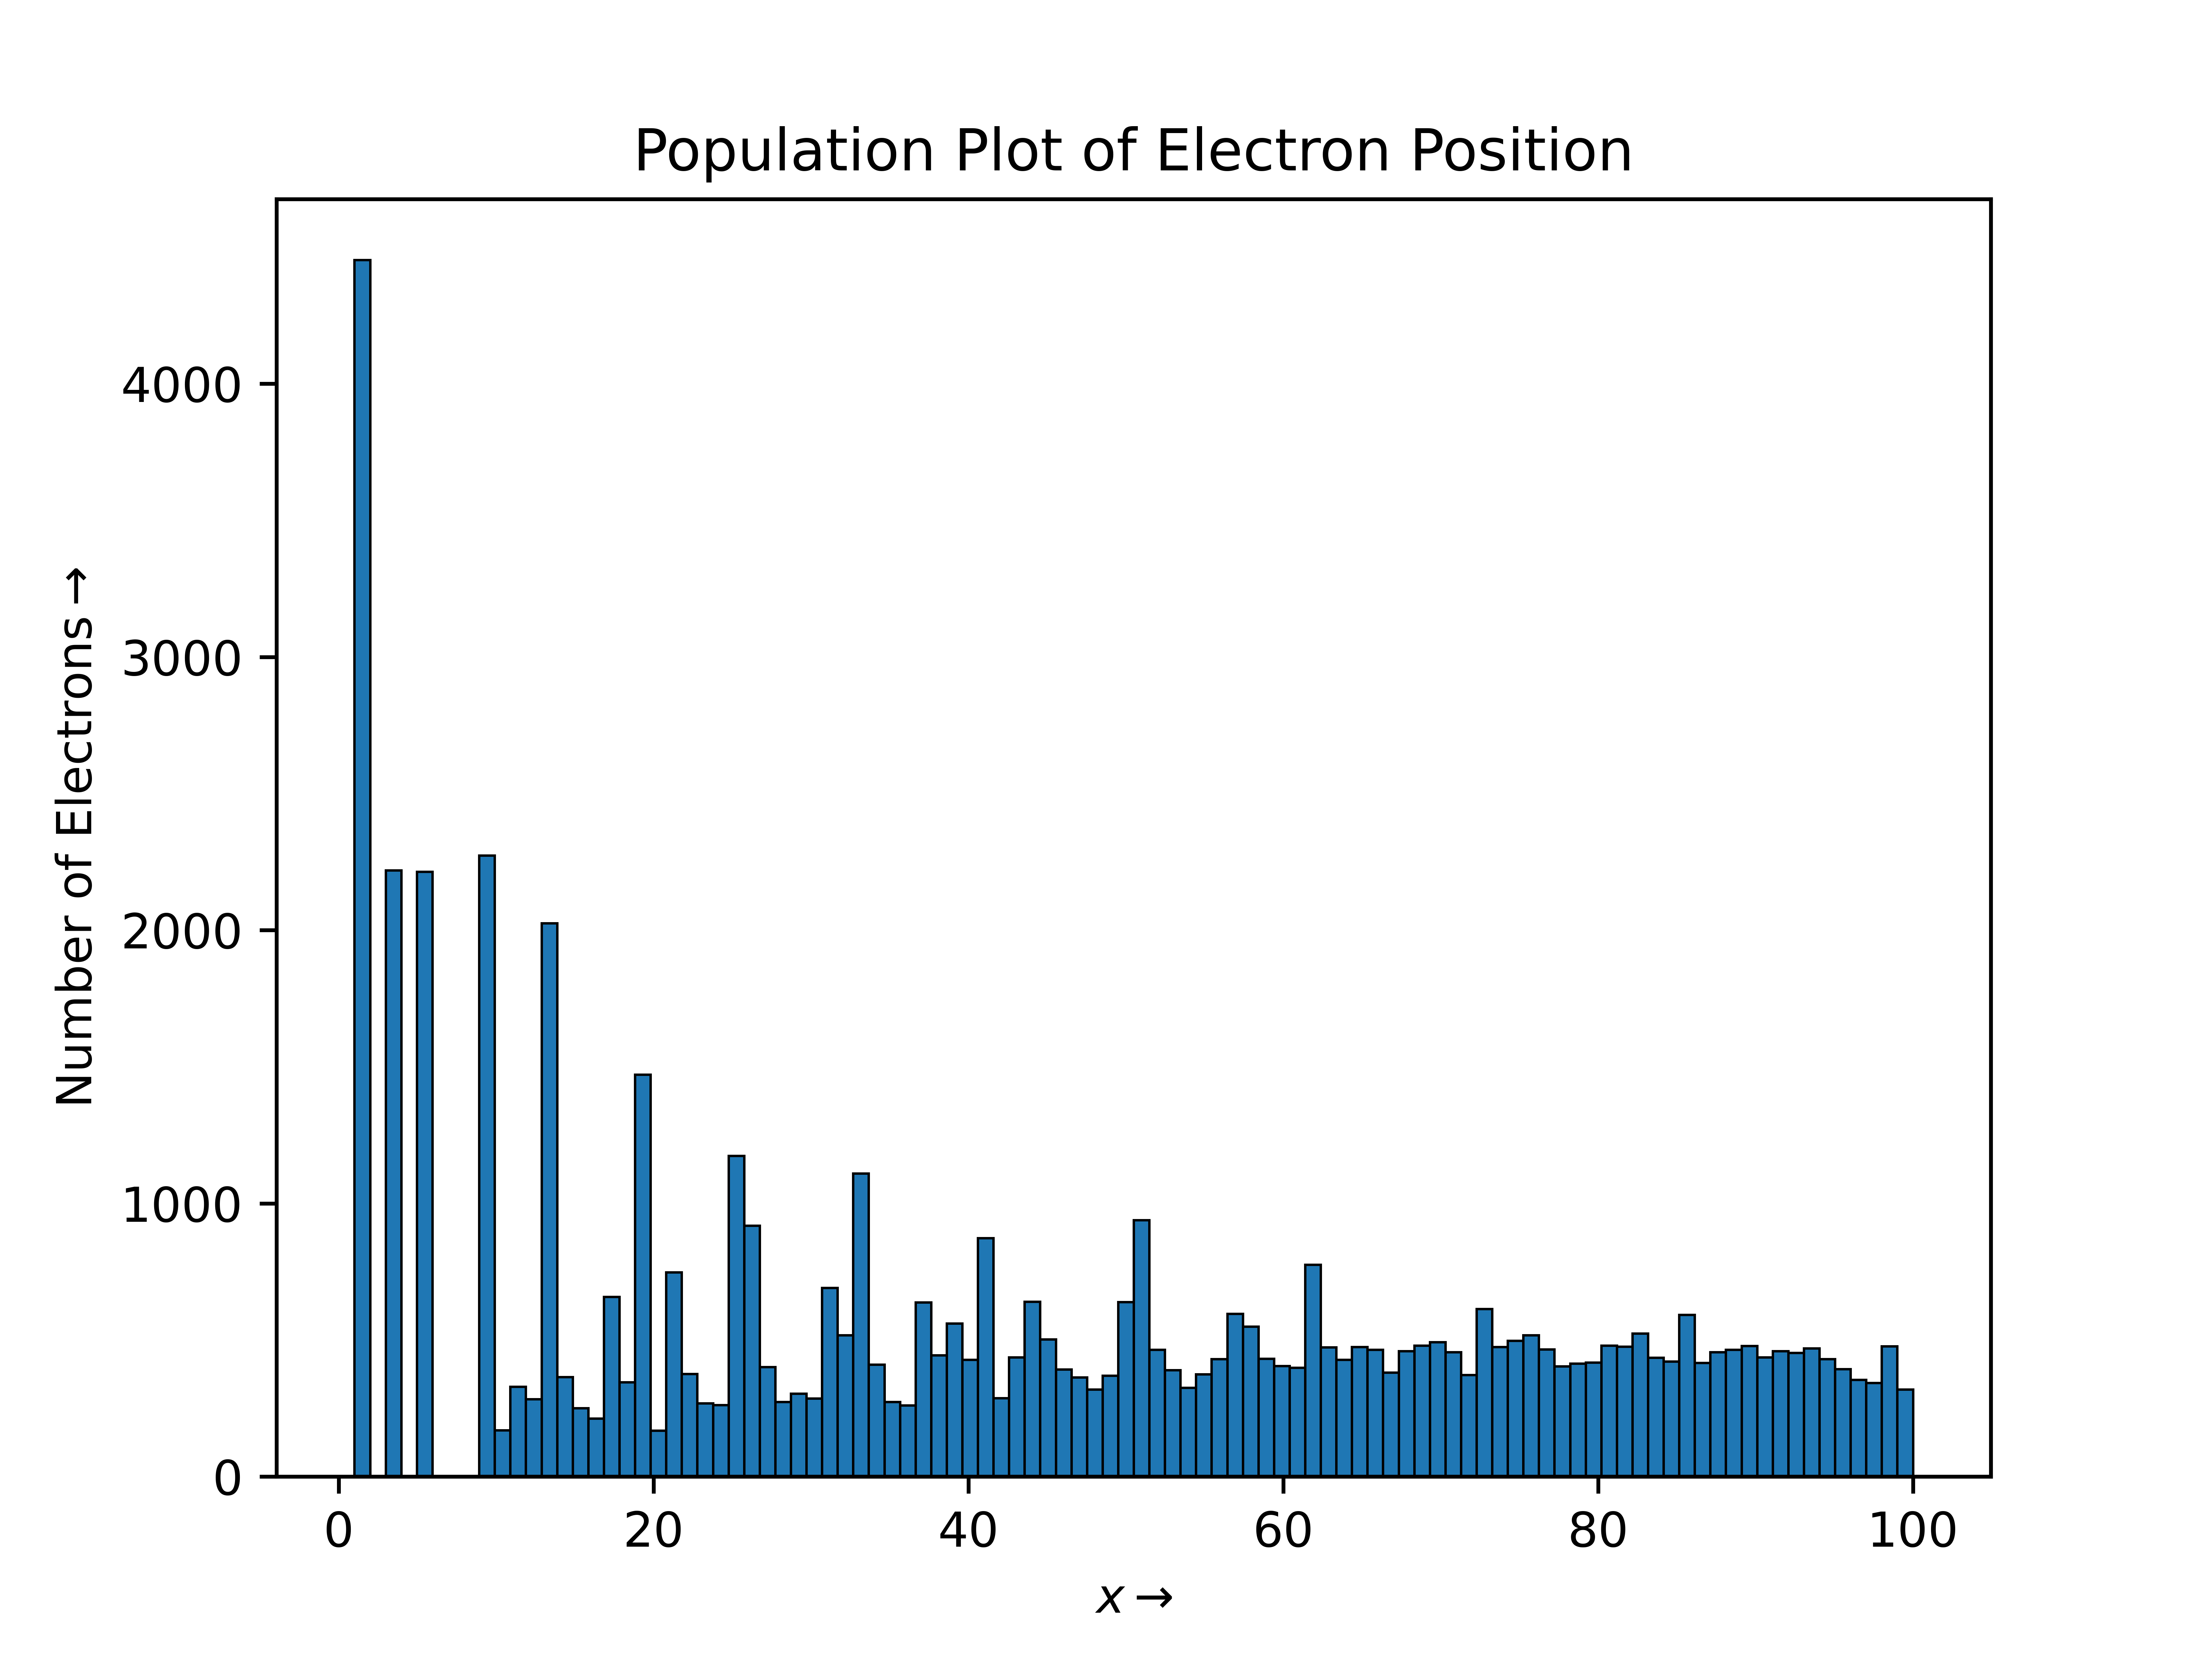
\includegraphics{images/fig0_acc.png}
    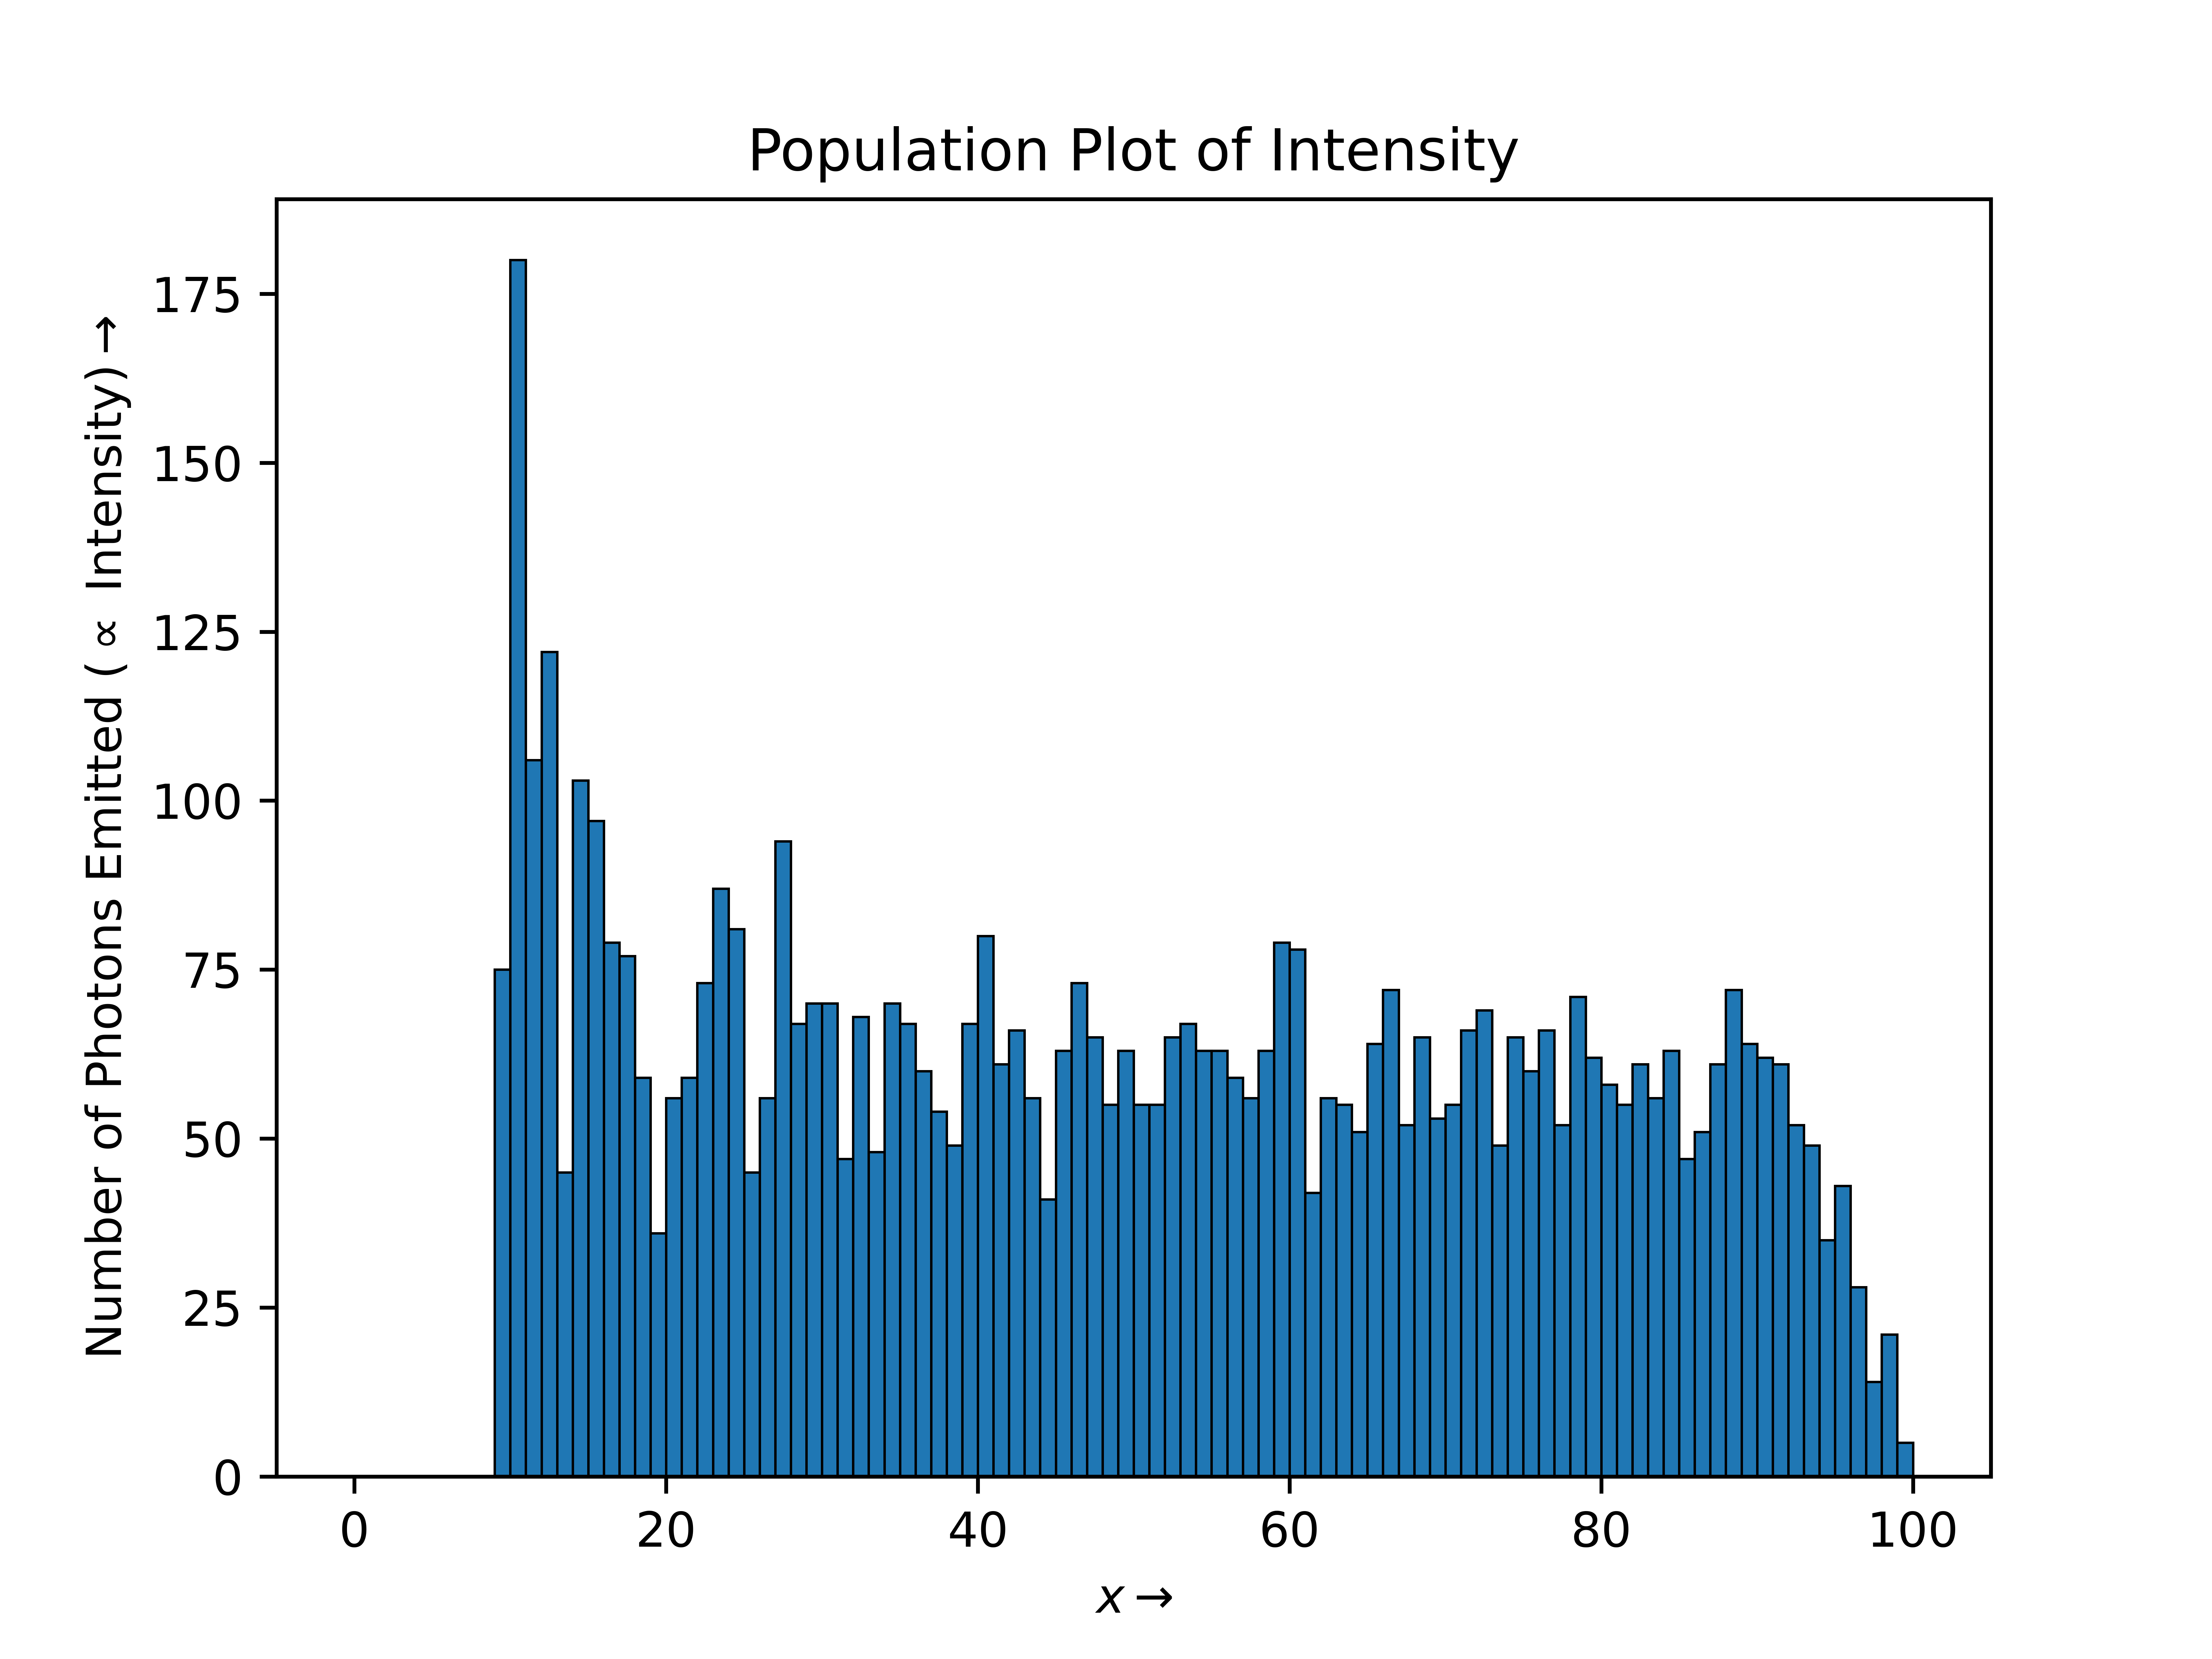
\includegraphics{images/fig1_acc.png}
\end{center}
\pagebreak
For the third graph I would like to change a few plotting parameters from before:

\begin{lstlisting}
plt.figure(2)
plt.scatter(X,V,marker='^',c='',edgecolor='red',linewidth=0.2)
plt.title("Electron Phase Space")
plt.xlabel("$x$")
plt.ylabel("$v$")
plt.savefig("images/fig2_acc.png",dpi=1000)
plt.show()
\end{lstlisting}

\begin{center}    
    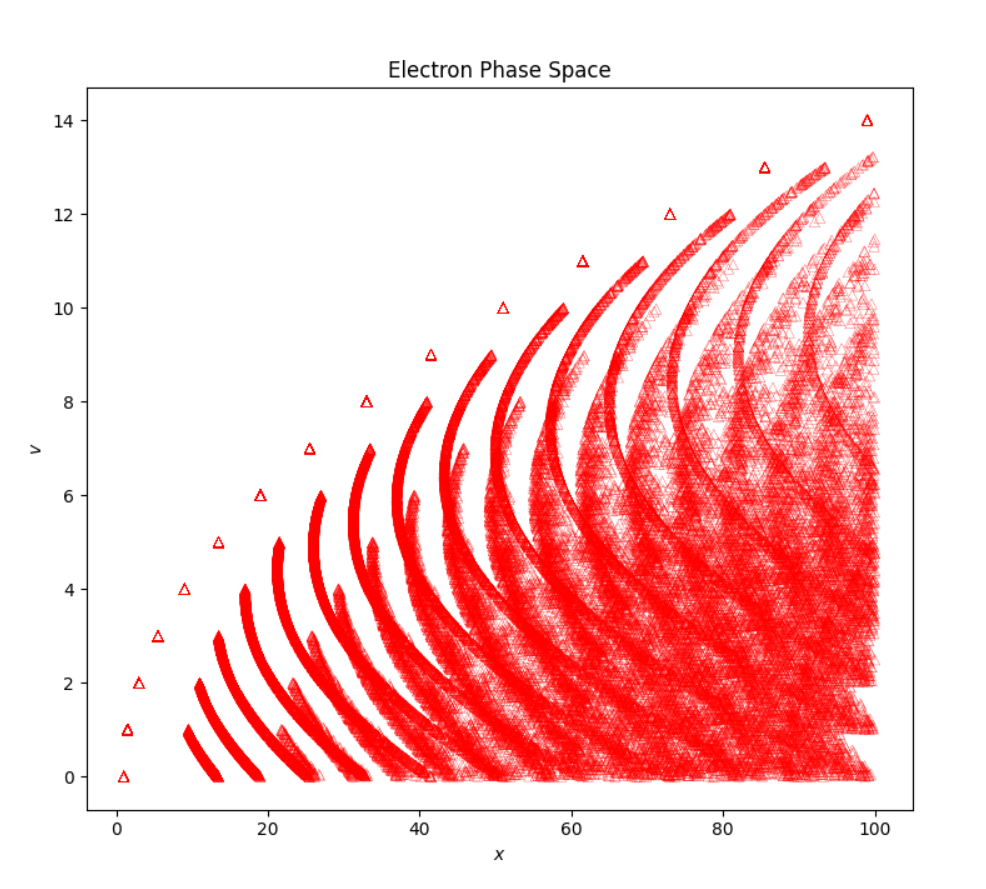
\includegraphics[width=\textwidth]{images/fig2_acc_1.png}
\end{center}
\pagebreak
\section{Conclusions from accurate graphs}
Now we see that the electron position and photon intensity are mostly unchanged, but the phase space now has continuous values of velocity. 

It also enables us to see families of curves, each of which corresponds to a peak in the photon density/emission intensity, corresponding to the number of collisions suffered by each of them.

It is still bounded by the parabolic envelope for the electrons that directly reach the anode from the cathode.

\end{document}
